\section{Relationship to the course (3 to 4 pages)}
% Summarize the themes/aspects from the lecture course which are relevant for the paper which you will discuss. 
% 
% 
% 
% \subsection{Van Wees}
% From the slides, reading material. Van Wees first because he was most fundamental about devices? Building up towards the more advanced organic stuff from Loi (as in the article).

% \begin{itemize}
% \item semionductor material, p-type, n-type
% \item FET (explain JFET, MOSFET)
% \item p-n junction / Schottky barrier (metal-semiconductor)
% \item LET (also use explanation from Box 1 in paper)
% \end{itemize}

\subsection{Transistors}

The ability to on a large scale produce transistors has been one of the biggest advancements in the 20th century. Transistors and derived devices are necessary components in every modern electronic device. They can amplify currents or switch the currents off completely. To make these transistors, one needs a material that can is capable of showing both characteristics of metals and of insulators, to be able to not only conduct currents, but also switch them off. These materials are called semiconductors, which have a band gap between the valence band and the conduction band. A pure semiconductor material behaves as an insulator, therefore doping of the material is needed to give it the metal-like properties.

Doping introduces either extra electrons (n-type doping) or extra holes (p-type doping) in a material. This is done by putting molecules with different covalent bond forming properties in the crystals. If the semiconductor is made from silicon, which forms 4 covalent bonds, to introduce extra electrons a material which forms 5 covalent bonds (e.g. arsenic) should be used. The extra electron is now only weakly bound to the ion, and new energy states are produced close to and below the conduction band. See also figure \ref{fig:ndoping}. For p-type doping a material that only forms 3 covalent bonds should be used. The `empty' place is a hole which can easily travel through the material. New acceptor states are produced just above the valence band (figure \ref{fig:pdoping}). [chapter 2.8 of Van Wees book]

\begin{figure}[!ht]
 \begin{center}
  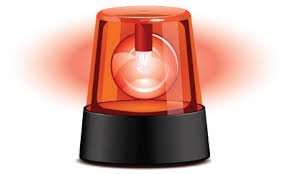
\includegraphics[width=0.8\textwidth]{alarm}
  \caption{}
  \label{fig:ndoping}
 \end{center}
\end{figure}

\begin{figure}[!ht]
 \begin{center}
  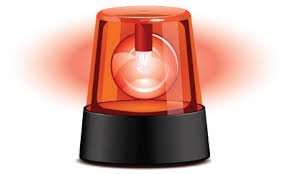
\includegraphics[width=0.8\textwidth]{alarm}
  \caption{}
  \label{fig:pdoping}
 \end{center}
\end{figure}

Therefore p-type semiconductors are semiconductors with holes the majority carriers, and n-type semiconductors have electrons as majority carriers.

Field-effect transistors are made of a combination of n-type and p-type semiconductors. The field effect refers to the control of the electrical conductivity of a material by the application of an external electric field. The working of a junction-FET (JFET) illustrates how this field effect is used.

\begin{figure}[!ht]
 \begin{center}
  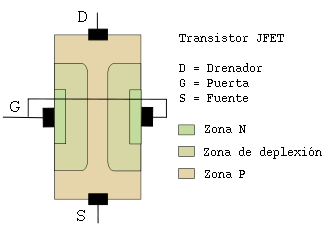
\includegraphics[width=0.8\textwidth]{JFET}
  \caption{A junction field effect transistor, with the position of source, drain and gate shown. A gate voltage influences the conductivity through the channel.}
  \label{fig:JFET}
 \end{center}
\end{figure}

In figure \ref{fig:JFET} a diagram of a JFET is shown. In this case the channel through which the charge carriers flow (with a voltage difference between source and drain), is made of an n-type semiconductor, and the surrounding substrate is made of a p-type semiconductor. Therefore the mobile charge carriers in the channel are electrons. When the holes in the substrate are pulled away by a negative voltage applied to the gate, a negatively charged area near the channel remains. This induces a negatively charged electric field, which penetrates into the channel and repels the electrons, effectively narrowing the channel. With a high enough gate voltage the channel can be completely `pinched' off, resulting in a voltage-controlled switch.

\subsubsection{Light emission}

-p-n junction, LED, LET

\subsection{Loi}
The Organic and optoelectronic part of the lecture is of most relevance to the paper. After the introduction into (inorganic) Light Emmitting Transistors the paper focuses on organic devices. 

\subsubsection{Tuneability}
One of the aspects from the lectures that is also covered in the paper is the tunabilty of organic semiconductors. With bulk inorganic semiconductor material it is not possible to change the bandgap a lot. Especially in light producing devices it is necessary to make nanocrystals. These nanocrystal structures are also needed for indirect bandgap meterials like silicon because they need a phonon to complete charge recombination. Without the nanocrystal structure the rocombination will occur via an non-radiative process. For organic semiconductors however it is relativly easy to change the bandgap. Most of the organic materials have a relative complex molecular structure compared to inorganic materials, therefore there are more possibilities to adjust the molecule slightly rusulting in different properties. 
\subsubsection{Easy and low-cost production}
An other advantage of organic semiconductors that is mentioned both in the lectures and in the article are the favorable production methods. Inorganic semiconductors require an expensive and complicated production method. (Iets uitleggen over litografie en etching etc) Organic semiconductors on the other hand can be easily printed from a solution. The solution can be printed on many different types of (cheaper) materials such as, glass, metal foils and plastics, which give the possibility of producing flexible semiconductors. Finally the costs of the organic semiconductor material itself is much cheaper and more widely available.
\subsubsection{Other differences between organic and inorganic devices}
-Mobility of charge
Mentioned briefly in both the paper and lectures is the mobility of charge carriers. For OLEDs the mobility is about 5 orders of magnitude lower than of inorganic LEDs. However the article describes a mobility for OLETs that can be 4 orders of magnitude higher, but still lower than that of inorganic materials.

-Lower efficiency for organic devices
However the efficiency of organic devices continues to increase it still is not at the level of inorganic devices for high brightness. The efficiency of light emitting devices is often described by the quantum efficiency. Which is defined as the "Fraction of excited carriers that recombine radiatively". And the equation is: $\eta = R_{r}/R = \tau_{nr}/(\tau_{tr}+\tau_{nr})$ Where $R=$ Total recombination rate, $R_{r}$=Radiative recombination rate, $\tau_{tr}=$Radiative lifetime, $\tau_{nr}=$Non-radiative lifetime. The goal is to have an as high as possible Radiative recombination rate. 

-Lower lifetime and higher vulnerability to the environment for OSC
Finally the lower lifetime of organic semiconductors is mentioned briefly. Organic semiconductors are more vulnorable to the environment because the organic materials react more easily with water or oxygen. Furthermore their lifetime is lower compared to inorganic semicunductors. 
